\section{Logic Circuits}

\underline{\textbf{Part 1 A}} \par

Build circuits consisting of a power supply, resistors, switches, and LEDs that obey the following logic: NOT, AND, and OR.
Make sure the current through any LEDs remains between 10 and 20 mA.
Safe values for voltage and resistance are approximately 2 $<$ V $<$ 4 V (DC) and 200 $<$ R $<$ 500 $\Omega$.  

\vspace{\baselineskip}

\underline{\textbf{Part 1 B}} \par

Construct a truth table for the 2-input, 2-output circuit shown below.

\begin{figure}[H]
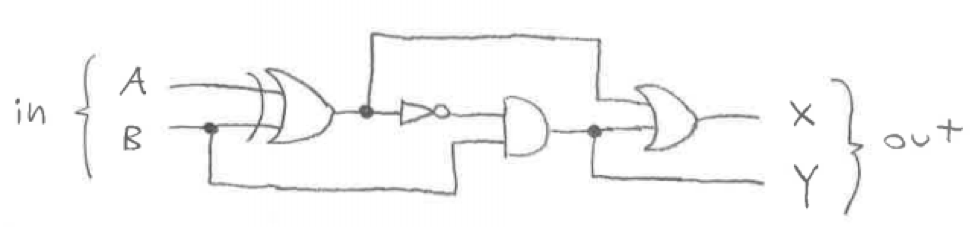
\includegraphics[scale=0.80]{figures/logic-circuits/fig1.png}
\end{figure}

\underline{\textbf{Part 2 A}} \par

Build NOT, AND, OR, and XOR circuits using a 4.5 V power supply, IC chips, resistors, and LEDs.
Note that the IC chips fit conveniently in the center of most breadboards as shown below and remember to use resistors in series with LEDs to keep the current between 10-20 mA.
Also note that a ``0'' input should be connected to ground (i.e. the negative side of your power supply), as opposed to being connected to nothing.
See the appendix for chip numbers.

\begin{figure}[H]
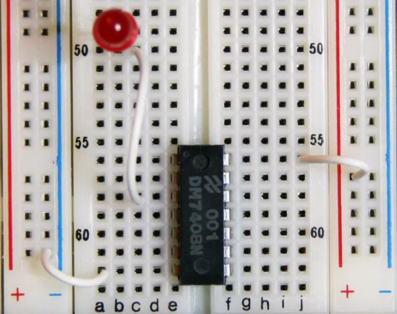
\includegraphics[scale=0.85]{figures/logic-circuits/fig2.png}
\end{figure}

Be very careful when removing the chips from the breadboards as the legs bend/break easily.
Avoid any unnecessary plugging and unplugging.
In order for the chips to function properly, pin 14 must be connected to +4.5 V and pin 7 must be connected to ground.
See below for pin numbers.

\vspace{\baselineskip}

The AND, OR, and XOR chips (below, left) each contain 4 gates while the NOT chips (below, right) contain 6 gates. 

\begin{figure}[H]
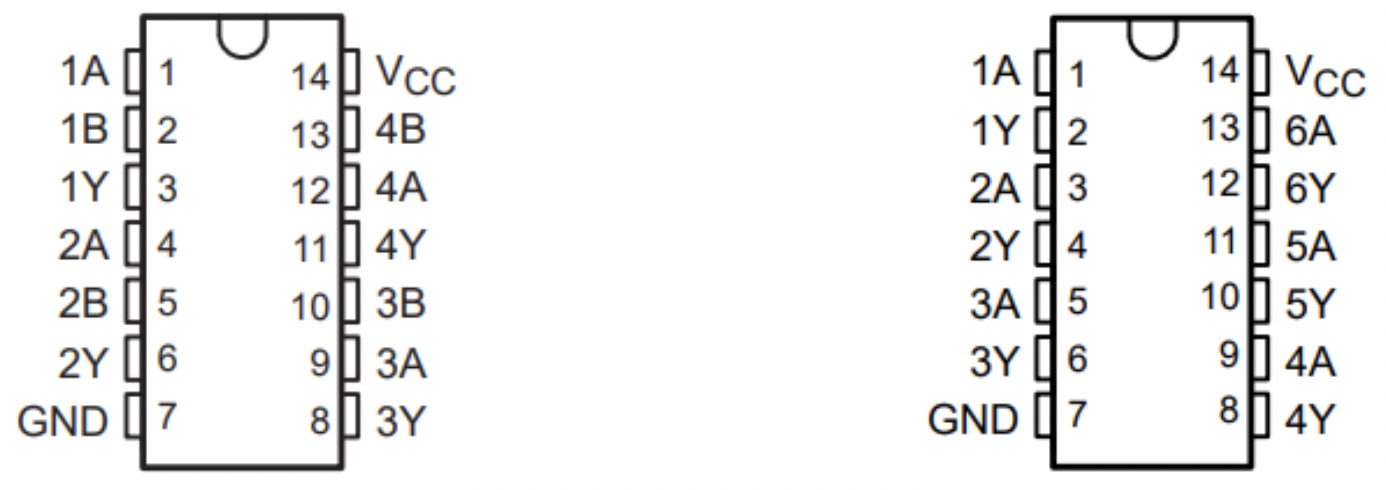
\includegraphics[scale=0.50]{figures/logic-circuits/fig3.png}
\end{figure}

In the above figures, A/B represent inputs and Y represents the output.
As an example, the figure below shows a more details picture of an OR chip.

\begin{figure}[H]
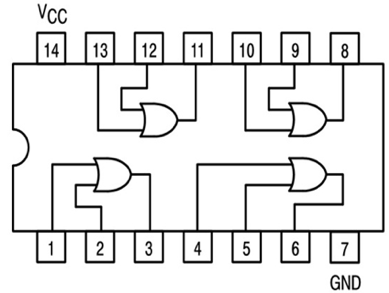
\includegraphics[scale=0.85]{figures/logic-circuits/fig4.png}
\end{figure}

\underline{\textbf{Part 2 B}} \par

Build the circuit below and confirm that it obeys XOR logic.

\begin{figure}[H]
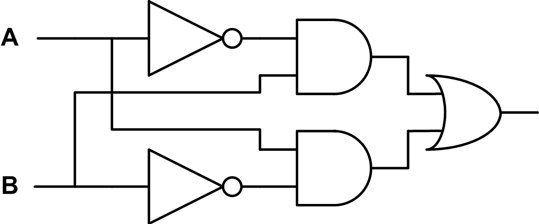
\includegraphics[scale=0.85]{figures/logic-circuits/fig5.png}
\end{figure}

\underline{\textbf{Part 2 C}} \par

Fill out the truth table for the following 2-input, 2-output circuit.
In the last column, consider XY a 2-digit binary number and convert it to decimal (i.e. base 10).
Build and test the circuit.
What did you just create?

\begin{figure}[H]
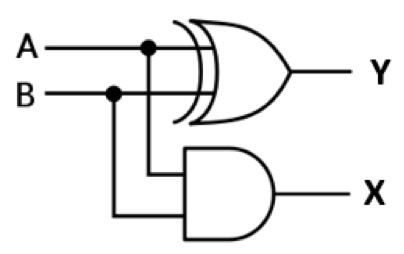
\includegraphics[scale=0.80]{figures/logic-circuits/fig6.png}
\end{figure}

\begin{tabular}[H]{ | c | c | c | c | c | }
\hline
A & B & X & Y & $\text{XY}_{10}$ \\
\hline
0 & 0 & \  & \  & \  \\
\hline
0 & 1 & \  & \  & \  \\
\hline
1 & 0 & \  & \  & \  \\
\hline
1 & 1 & \  & \  & \  \\
\hline
\end{tabular}

\vspace{\baselineskip}

\underline{\textbf{Appendix}} \par

\vspace{\baselineskip}

OR: 296-1615-5-ND/SN74HCT32N \\
XOR: 296-4777-5-ND/SN74AHCT86N \\
AND: 296-1606-5-ND/SN74HCT08N \\
NOT: 296-1605-5-ND/SN74HCT04N

\pagebreak \clearpage
